\documentclass[a4paper,11pt]{article}
\usepackage{blindtext}
\usepackage[top=1in,left=0.5in,right=0.5in,bottom=1in]{geometry}
\usepackage[utf8]{inputenc}
\usepackage[T1]{fontenc}
\usepackage{graphicx}
\usepackage{verbatim}
\usepackage{array}
\usepackage{rotating}
\usepackage{caption}
\usepackage{multicol}
\usepackage{amsmath}
\usepackage{amsfonts}
\usepackage[toc,page]{appendix}
\usepackage{amsthm}
\usepackage{amssymb}
\usepackage{empheq}
\usepackage{listings}
\usepackage{tikz}
\usetikzlibrary{arrows, calc, shapes.multipart, chains, positioning, arrows.meta, bending}
\usepackage{xcolor}
\usepackage{fancyhdr}
\usepackage{setspace}
\usepackage{mathtools}
\usepackage{esdiff}
\usepackage{multirow}
\usepackage[default,scale=0.95]{opensans}

%increase table row heights
\renewcommand{\arraystretch}{1.25}

%all displaystyle
\everymath{\displaystyle}

%equation numbers
\newcommand\numberthis{\addtocounter{equation}{1}\tag{\theequation}}

%ceil and floor
\providecommand{\ceil}[1]{\left \lceil #1 \right \rceil }
\providecommand{\floor}[1]{\left \lfloor #1 \right \rfloor }

%no space mod
\newcommand{\Mod}[1]{\ (\mathrm{mod}\ #1)}

\tikzset{
	outernode/.style={draw,thick, inner sep=0},
	innernode/.style={inner sep=.3333em, draw, rectangle split, rectangle split parts=#1}
}
\tikzstyle{rect} = [thick, rectangle, text centered, minimum size=18pt, inner sep=5pt, text=black, draw=black, fill=white]

%New colors defined below
\definecolor{codegreen}{rgb}{0,0.6,0}
\definecolor{codegray}{rgb}{0.5,0.5,0.5}
\definecolor{codepurple}{rgb}{0.58,0,0.82}
\definecolor{backcolour}{rgb}{0.95,0.95,0.92}

%Code listing style named "mystyle"
\lstdefinestyle{mystyle}{
	backgroundcolor=\color{backcolour},   commentstyle=\color{codegreen},
	keywordstyle=\color{magenta},
	numberstyle=\tiny\color{codegray},
	stringstyle=\color{codepurple},
	basicstyle=\ttfamily\footnotesize,
	breakatwhitespace=false,         
	breaklines=true,                 
	captionpos=b,                    
	keepspaces=true,                 
	numbers=left,                    
	numbersep=5pt,                  
	showspaces=false,                
	showstringspaces=false,
	showtabs=false,                  
	tabsize=2
}

%"mystyle" code listing set
\lstset{style=mystyle}

%Remove indentation to all paragraph
\setlength{\parindent}{0pt}

%Better square root
\usepackage{letltxmacro}
\makeatletter
\let\oldr@@t\r@@t
\def\r@@t#1#2{%
	\setbox0=\hbox{$\oldr@@t#1{#2\,}$}\dimen0=\ht0
	\advance\dimen0-0.2\ht0
	\setbox2=\hbox{\vrule height\ht0 depth -\dimen0}%
	{\box0\lower0.4pt\box2}}
\LetLtxMacro{\oldsqrt}{\sqrt}
\renewcommand*{\sqrt}[2][\ ]{\oldsqrt[#1]{#2}}
\makeatother

\newcommand*\dd{\mathop{}\!\mathrm{d}} 

\makeatletter
\renewcommand*\env@matrix[1][*\c@MaxMatrixCols c]{%
	\hskip -\arraycolsep
	\let\@ifnextchar\new@ifnextchar
	\array{#1}}
\makeatother

\newcommand{\grad}{\nabla}
\newcommand{\divr}{\nabla \cdot}
\newcommand{\curl}{\nabla \times}
\newcommand{\bvec}[1]{\mathbf{#1}}
\newcommand{\bhat}[1]{\hat{\mathbf{#1}}}
\newcommand{\uvec}[1]{\hat{\mathbf{a}}_{#1} }

%\pagestyle{fancy}
%\fancyhf{}
%\rhead{Math 40 - WFY | Julius Basilla}
%\chead{2019-04243}
%\lhead{Mesa, Allan Jr. J.}
%\rfoot{Page \thepage}

\title{\textbf{EEE 135 Key concepts and Equations}}
\author{AJ Mesa Jr.}

\begin{document}
	\maketitle	
	\section*{Vectors}
		\begin{enumerate}
			\item $\bvec{A} \times (\bvec{B} \times \bvec{C}) = \bvec{B}(\bvec{A} \cdot \bvec{C}) - \bvec{C}(\bvec{A} \cdot \bvec{B} )$
			\item $(\bvec{A} \times \bvec{B}) \times \bvec{C} = -\bvec{A}(\bvec{B} \cdot \bvec{C}) + \bvec{B}(\bvec{A} \cdot \bvec{C} )$
			\item $\bvec{A} \cdot (\bvec{B} \times \bvec{C}) = \bvec{B} \cdot (\bvec{C} \times \bvec{A}) = \bvec{C} \cdot (\bvec{A} \times \bvec{B}) = \left| \bvec{A}\bvec{B}\bvec{C} \right|$
			\item $\grad(\bvec{A} \times \bvec{B}) = (\grad \times \bvec{A})\cdot\bvec{B} - (\grad \times \bvec{B})\cdot\bvec{A}$
			\item $\grad\times (\bvec{A} \times \bvec{B}) = \bvec{A}(\divr\bvec{B}) - \bvec{B}(\divr\bvec{A}) + \bvec{A}(\bvec{B}\cdot\grad) - \bvec{B}(\bvec{A}\cdot\grad)$
			\item $\divr(\curl\bvec{A}) = 0$ 
			\item $\curl(\grad A) = \bvec{0}$
			\item $\divr(\grad\phi) = \grad^2\phi$
			\item $\grad(\divr\bvec{A}) - \curl(\curl\bvec{A}) = \grad^2 \bvec{A}$
			\item Divergence theorem: $\displaystyle \oint\displaylimits_\text{closed surface} \bvec{A} \cdot \dd \bvec{S} = \int\displaylimits_\text{volume bounded} (\divr\bvec{A}) \dd v$
			\item Stokes' theorem: $\displaystyle \oint\displaylimits_\text{closed loop} \bvec{A} \cdot \dd \bvec{L} = \int\displaylimits_\text{surface bounded} (\curl\bvec{A}) \cdot \dd \bvec{S} $
		\end{enumerate}
	\newpage
	\section*{Coordinate Systems}
		\begin{tabular}{|l|c|c|c|}
			\hline
			& Rectangular & Cylindrical & Spherical \\ \hline
			\multirow{3}{*}{Parameters} & $x$ & $\rho = \sqrt{x^2 + y^2}$ & $r = \sqrt{x^2 + y^2 + z^2}$ \\
			& $y$ & $\displaystyle\phi = \arctan\left(\frac{y}{x}\right)$ & $\displaystyle\phi = \arctan\left(\frac{y}{x}\right)$ \\
			& $z$ & $z$  & $\displaystyle \theta = \arctan \left( \frac{\sqrt{x^2 + y^2}}{z} \right)$ \\ \hline
			\multirow{3}{*}{Conversion} & & $x = \rho\cos\phi$ & $x = (r\sin\theta)\cos\phi$ \\ 
			& & $y = \rho\sin\phi$ & $y = (r\sin\theta)\sin\phi$ \\
			& & $z = z$ & $z = r\cos\theta$ \\ \hline
			\multirow{3}{*}{Unit Vectors} & $\bhat{a}_x$ & $\bhat{a}_\rho = \uvec{x}\cos\phi + \uvec{y}\sin\phi$ & $\bhat{a}_r = \uvec{x}\sin\theta\cos\phi + \uvec{y}\sin\theta\sin\phi + \uvec{z}\cos\theta$ \\
			& $\bhat{a}_y$ & $\bhat{a}_\phi = -\uvec{x}\sin\phi + \uvec{y}\cos\phi$ & $\bhat{a}_\phi = -\uvec{x}\sin\phi + \uvec{y}\cos\phi$ \\
			& $\bhat{a}_z$ & $\bhat{a}_z$ & $\bhat{a}_\theta = \uvec{x}\cos\theta\cos\phi + \uvec{y}\cos\theta\sin\phi - \uvec{z}\sin\theta$ \\ \hline
			$\dd v$ & $\dd x \dd y \dd z$ & $\dd \rho (\rho \dd \phi) \dd z$ & $\dd r (r\dd\phi)(r\sin\theta \dd\theta)$ \\ \hline
			$\dd\bvec{L}$ & $\dd x \uvec{x} + \dd y \uvec{y} + \dd z \uvec{z}$ & $\dd \rho \uvec{\rho} + \rho\dd \phi \uvec{\phi} + \dd z \uvec{z}$ & $\dd r \uvec{r} \uvec{r} + r\dd \theta \uvec{\theta} + r\sin\theta\dd \phi \uvec{\phi}$ \\ \hline
			Vector Field & $A_x\bhat{a}_x + A_y\bhat{a}_y + A_z\bhat{a}_z$ & $A_\rho\uvec{\rho} + A_\phi\uvec{\phi} + A_z\uvec{z}$ & $A_\rho\uvec{\rho} + A_\phi\uvec{\phi} + A_\theta\uvec{\theta}$\\ \hline 
			$\grad A$& $\displaystyle \diffp{A}{x}\uvec{x} + \diffp{A}{y}\uvec{y} + \diffp{A}{z}\uvec{z}$ & $\displaystyle \diffp{A}{\rho}\uvec{\rho} + \frac{1}{\rho}\diffp{A}{\phi}\uvec{\phi} + \diffp{A}{z}\uvec{z}$ & $\displaystyle \diffp{A}{r}\uvec{r} + \frac{1}{r}\diffp{A}{\theta}\uvec{\theta} + \frac{1}{r\sin\theta}\diffp{A}{\phi}\uvec{\phi}$ \\ \hline
			\multirow{2}{*}{$\divr \bvec{A}$} & $\displaystyle \diffp{A_x}{x} + \diffp{A_y}{y} + \diffp{A_z}{z}$ & $\displaystyle \frac{1}{\rho}\diffp{(\rho A_\rho)}{\rho} + \frac{1}{\rho}\diffp{A_\phi}{\phi} $ & $\displaystyle \frac{1}{r^2}\diffp{(r^2 A_r)}{r} + \frac{1}{r\sin\theta}\diffp{A_\phi}{\phi}$ \\
			& & $\displaystyle +\diffp{A_z}{z}$ & $\displaystyle +\frac{1}{r\sin\theta}\diffp{(A_\theta \sin\theta)}{\theta}$ \\ \hline
			\multirow{3}{*}{$\curl\bvec{A}$} & $\displaystyle \left(\diffp{A_z}{y} - \diffp{A_y}{z}\right)\uvec{x}$ & $\displaystyle \left(\frac{1}{\rho}\diffp{A_z}{\rho} - \diffp{A_\phi}{z}\right)\uvec{\rho}$ & $\displaystyle \frac{1}{r\sin\theta}\left(\diffp{(A_\phi\sin\theta)}{\theta} - \diffp{A_\theta}{\phi}\right)\uvec{r}$ \\
			& $\displaystyle + \left(\diffp{A_x}{z} - \diffp{A_z}{x}\right)\uvec{y}$ & $\displaystyle \left(\diffp{A_\rho}{z} - \diffp{A_z}{\rho}\right)\uvec{\rho}$ & $\displaystyle \frac{1}{r}\left(\frac{1}{\sin\theta}\diffp{A_r}{\phi} - \diffp{(rA_\phi)}{r}\right)\uvec{\theta}$ \\  
			& $\displaystyle + \left(\diffp{A_y}{x} - \diffp{A_x}{y}\right)\uvec{z}$ & $\displaystyle \frac{1}{\rho}\left(\diffp{(\rho A_\phi)}{\rho} - \diffp{A_\rho}{\phi}\right)\uvec{z}$ & $\displaystyle \frac{1}{r}\left(\diffp{(rA_\theta)}{r} - \diffp{(A_r)}{\theta}\right)\uvec{\phi}$ \\ \hline
			\multirow{2}{*}{$\grad^2 A$} & $\displaystyle \diffp[2]{A_x}{x} + \diffp[2]{A_y}{y} + \diffp[2]{A_z}{z}$ & $\displaystyle \frac{1}{\rho} \diffp{}{\rho} \left(\rho\diffp{A}{\rho}\right) + \frac{1}{\rho^2} \diffp[2]{A}{\phi}$& $\displaystyle \frac{1}{r^2} \diffp{}{r}\left(r\diffp{A}{r}\right) + \frac{1}{r^2\sin^2\theta}\diffp[2]{A}{\phi}$\\
			& & $ + \diffp[2]{A_z}{z}$ & $+ \displaystyle \frac{1}{r^2\sin\theta} \diffp{}{\theta} \left(\sin\theta\diffp{A}{\theta}\right)$ \\ \hline
		\end{tabular} \\
	\vspace{10mm}
	\newline 
	Unit vector dot products: 
		\begin{multicols}{2}
			\begin{enumerate}
				\item rectangular and cylindrical:\\ 
				\begin{tabular} {|l|c|c|c|} \hline
					& $\uvec{\rho}$ & $\uvec{\phi}$ & $\uvec{z}$ \\ \hline
					$\uvec{x}$ & $\cos\phi$ & $-\sin\phi$ & $0$ \\ \hline
					$\uvec{y}$ & $\sin\phi$ & $\cos\phi$ & $0$ \\ \hline
					$\uvec{z}$ & $0$ & $0$ & $1$ \\ \hline
				\end{tabular}
				\item rectangular and spherical:\\ 
				\begin{tabular} {|l|c|c|c|} \hline
					& $\uvec{r}$ & $\uvec{\phi}$ & $\uvec{\theta}$ \\ \hline
					$\uvec{x}$ & $\sin\theta\cos\phi$ & $-\sin\phi$ & $\cos\theta\cos\phi$ \\ \hline
					$\uvec{y}$ & $\sin\theta\sin\phi$ & $\cos\phi$ & $\cos\theta\sin\phi$ \\ \hline
					$\uvec{z}$ & $\cos\theta$ & $0$ & $-\sin\theta$ \\ \hline
				\end{tabular}
			\end{enumerate}
		\end{multicols} 	
	
	\newpage
	\section{Electrostatics}
	\begin{enumerate}
		\item Coulomb's law, the force between two charged particles: $\displaystyle \bvec{F}_2 = \frac{1}{4\pi\varepsilon_0}\frac{Q_1Q_2}{r^2}\uvec{12}$ with $\frac{\bvec{r}_2 - \bvec{r}_1}{ \left|\bvec{r}_2 - \bvec{r}_1\right|}$
		\item electric field intensity of charge $Q$ is force per unit charge: $\bvec{E} = \frac{\bvec{F}_t}{Q_t} = \frac{1}{4\pi\varepsilon_0}\frac{Q_1}{r^2}\uvec{r} $
		\item volume charge density: $\rho_v = \lim_{\Delta v \to 0} \frac{\Delta Q}{\Delta v} = \diff{Q}{v} \Longleftrightarrow Q = \int\limits_\text{volume} \rho_v \dd v$ 
		\item field of line charge: $\bvec{E} = \frac{\rho_L}{2\pi\varepsilon_0\rho}\uvec{\rho}$
		\item field of sheet charge: $\bvec{E} = \frac{\rho_S}{2\varepsilon_0}\uvec{N}$
		\item sketching streamlines: $\frac{E_y}{E_x} = \diff{y}{x}$
		\item electric flux = induced charge of conductor on another (grounded) without contact: $\Psi = Q$
		\item electric flux density = electric flux per unit area: $\bvec{D} = \frac{Q}{4\pi r^2}\uvec{r} = \int\limits_\text{volume} \frac{\rho_v \dd v}{4\pi r^2} \uvec{r}$
		\item in free space: $\bvec{D} = \varepsilon_0\bvec{E}$
		\item Gauss's law: the electric flux passing through any closed surface is equal to the total enclosed charge by the surface. $\Psi = \int \dd \Psi = \oint\limits_\text{closed surface} \bvec{D}_s \cdot \dd \bvec{S} = Q = \int \rho_v \dd v$
		\item we apply Divergence theorem: $\oint\limits_\text{closed surface} \bvec{D}_s \cdot \dd \bvec{S} = \int (\divr\bvec{D}) \dd v = \int \rho_v \dd v \Longleftrightarrow \divr \bvec{D} = \rho_v$
		\item point form of Gauss's law: $\boxed{\divr \bvec{D} = \rho_v}$
		\item the work done by an external force to move a charge: $W = -Q\int\limits_\text{initial}^\text{final} \bvec{E} \cdot \dd \bvec{L}$ 
		\item potential difference = work done by external force per unit charge: $V = -\int\limits_\text{initial}^\text{final} \bvec{E} \cdot \dd\bvec{L}$
		\item potential difference is path independent, and $\oint \bvec{E} \cdot \dd\bvec{L} = 0$ 
		\item relationship of potential and electric field: $\bvec{E} = -\grad V$
		\item using the curl of divergence is 0: $\curl\bvec{E} = \curl(-\grad V) = \bvec{0}$
		\item Maxwell's $2$nd equation: $\boxed{\curl\bvec{E} = \bvec{0}}$
		\item electric dipole: two point charges of same magnitude, opposite charge and has a fixed distance 
		\item dipole moment: $\bvec{p} = Q\bvec{d}$ where $\bvec{d}$ points from $-Q$ to $+Q$
		\item torque on dipole by electric field: $\dd\bvec{T} = \dd\bvec{p}\times\bvec{E}$
		\item potential energy of dipole on electric field: $U = -\dd\bvec{p}\cdot\bvec{E}$
		\item total energy of system of $N$ charges: $W_E = \frac{1}{2}\sum_{n = 1}^{n = N}Q_nV_n$
		\item for continuous charge distribution: $W_E = \frac{1}{2}\int\limits_\text{volume} \rho_v V \dd v = \frac{1}{2}\int\limits_\text{volume} \bvec{D} \cdot \bvec{E} \dd v = \frac{1}{2}\int\limits_\text{volume} \varepsilon E^2 \dd v$
		\item energy density: $\diff{W_E}{v} = \frac{1}{2}\bvec{D}\cdot\bvec{E}$
	\end{enumerate}

	\section{Conductors and Dielectrics, Capacitance}
	\begin{enumerate}
		\item current = charges passing through an area per unit time: $I = \diff{q}{t}$ 
		\item current density = current per area: $I = \oint\limits_{S} \bvec{J} \cdot \dd \bvec{S}$
		\item let $Q_i$ be the charge flowing OUT a surface. the continuity equation: $\oint\limits_S \bvec{J}\cdot\dd\bvec{S} = -\diff{Q_i}{t}$
		\item point form of continuity equation: $\divr \bvec{J} = \diffp{\rho_v}{t}$
		\item electron drift speed: $\bvec{v}_d = -\mu_e\bvec{E}$ with $\mu$ = mobility 
		\item conductivity: $\sigma_e = -\rho_e\mu_e$
		\item vector form of Ohm's law: $\bvec{J} = \sigma\bvec{E}$
		\item Ohm's law: $V = IR$ 
		\item resistance $R = \frac{L}{\sigma S} = \frac{V_{ab}}{I} = \frac{-\int_b^a \bvec{E} \cdot\dd\bvec{L}}{\int_{S} \bvec{E} \cdot \dd\bvec{S}}$
		\item boundary conditions for conductors:
			\begin{itemize}
				\item $D_t = E_t = 0$
				\item $D_N = \varepsilon\bvec{E}_N = \rho_s$
				\item there is no field inside
				\item the field on the surface is normal to the surface
				\item the surface is an equipotential surface
			\end{itemize}
		\item Method of Images: the effect of an infinite conducting sheet is the same as the effect of the sheet removed and all other charges reflected with respect to the sheet.
		\item semiconductors: there is contribution of both electrons ansd holes $\sigma = -\rho_e\mu_e + \rho_h\mu_h$ 
		\item polarization = dipole moment per unit volume: $\bvec{P} = \lim_{\Delta v \to 0} \frac{1}{\Delta v} \sum_{i = 1}^{n\Delta b} \bvec{p}_i$
		\item total bounded charges: $Q_b = -\oint_S \bvec{P} \cdot \dd \bvec{S}$
		\item total free charges: $Q = Q_T - Q_b = \oint_S(\varepsilon_0\bvec{E} + \bvec{P})\cdot  \dd\bvec{S}$
		\item linear relationship of $\bvec{P}$ and $\bvec{E}$: $\bvec{P} = \chi_e\varepsilon_0\bvec{E}$ where $\chi_e$ is the electric susceptibility of the material
		\item relative permittivity: $\varepsilon_r = \chi_e + 1$
		\item permitivity: $\varepsilon = \varepsilon_0\varepsilon_r$
		\item in polarizable material: $\bvec{D} = \varepsilon_0\bvec{E} + \bvec{P} = \varepsilon_0\bvec{E}(1 + \chi_e) = \varepsilon\bvec{E}$
		\item boundary conditions for perfect dielectric materials: 
			\begin{itemize}
				\item $E_{t,~1} = E_{t,~2} \Longleftrightarrow (\bvec{E}_1 - \bvec{E}_2) \times \bhat{n} = 0$
				\item $\frac{D_{t,~1}}{D_{t,~2}} = \frac{\varepsilon_1}{\varepsilon_2}$
				\item $D_{N,~1} = D_{N,~2} \Longleftrightarrow (\bvec{D}_1 - \bvec{D}_2) \cdot \bhat{n} = \rho_S$
				\item $\varepsilon_1E_{N,~1} = \varepsilon_2E_{N,~2}$
				\item $D_2 = D_1 \sqrt{\cos^2\theta_1 + \left(\frac{\varepsilon_1}{\varepsilon_2}\right)^2\sin^2\theta_1}$ 
				\item $E_2 = E_1 \sqrt{\sin^2\theta_1 + \left(\frac{\varepsilon_1}{\varepsilon_2}\right)^2\cos^2\theta_1}$ 
			\end{itemize}
		\item capacitance: dependent only on the geometry of the capacitor: $C = \frac{\oint_S \varepsilon\bvec{E} \cdot \dd \bvec{S}}{-\int_-^+ \bvec{E} \cdot \dd\bvec{L}}$	
		\item parallel plate: $C = \frac{\varepsilon S}{d}$
		\item cylindrical capacitor: $C = \frac{2\pi\varepsilon L}{\ln\left(\frac{b}{a}\right)}$
		\item spherical capacitor: $C = 4\pi\varepsilon \left(\frac{1}{a} - \frac{1}{b}\right)^{-1}$
		\item Poisson equation: $\grad^2 V = -\frac{\rho_v}{\varepsilon}$
		\item Laplace equation: $\grad^2 V = 0$
	\end{enumerate}

	\section{Magnetostatics}
	\begin{enumerate}
		\item Biot-Savart law: $\dd\bvec{H} = \frac{I \dd \bvec{L} \times \uvec{r}}{4\pi r^2}$
		\item magnetic field intensity $\bvec{H}$ is analogous to electric field
		\item only the integral form has experimental basis: $\bvec{H} = \oint \frac{I\dd\bvec{L}\times\uvec{r}}{4\pi r^2} = \oint \frac{K\times\uvec{r}\dd S}{4\pi r^2} = \oint \frac{J\times\uvec{r}\dd v}{4\pi r^2}$
		\item surface current density: $I\dd\bvec{L} = \bvec{K}\dd S = \bvec{J} \dd v$
		\item Ampere's circuital law: $\oint \bvec{H} \cdot \dd \bvec{L} = I$
		\item point form of Ampere's circuital law: $\boxed{\curl\bvec{H} = \bvec{J}}$
		\item magnetic flux density = magnetic flux per area (in free space): $\bvec{B} = \mu_0\bvec{H}$
		\item magnetic flux: $\Phi = \int_S \bvec{B}\cdot\dd\bvec{S}$
		\item for a closed surface: $\Phi = \oint_S \bvec{B}\cdot\dd\bvec{S} = 0$
		\item using divergence theoren: $\oint_S \bvec{B}\cdot\dd\bvec{S} = \int\limits_\text{volume} (\divr \bvec{B}) \dd v = 0$
		\item point form of magnetic flux: $\boxed{\divr \bvec{B} = 0}$
		\item Maxwell's equations for static fields: \\
			\begin{center}
			\begin{tabular}{|c|c|}
				\hline
				Differential & Integral \\ \hline
				$\divr \bvec{D} = \rho_v$ & $\oint_S \bvec{D} \cdot \dd\bvec{S} = Q$ \\
				$\curl \bvec{E} = \bvec{0}$ & $\oint \bvec{E} \cdot \dd \bvec{L} = 0$\\
				$\curl \bvec{H} = \bvec{J}$ & $\oint \bvec{H} \cdot \dd \bvec{L} = I$\\
				$\divr \bvec{B} = 0$ & $\oint_S \bvec{B} \cdot \dd \bvec{S} = 0$ \\ \hline
			\end{tabular}
			\end{center}
		\item Scalar magnetic potential: we designate a scalar magnetic potential similar to electric potential such that $\bvec{H} = -\grad V_m (\text{when} \bvec{J} = \bvec{0})$ because the curl of a gradient is $0$. 
		\item this scalar magnetic potential obey's Laplace's equation: $\grad^2 V_m = 0$
		\item however, this potential is NOT CONSERVATIVE. $V_{m,~ab} = -\int_{b}^{a} \bvec{H} \cdot\dd\bvec{L},~\oint\bvec{H}\cdot\dd\bvec{L} = I \neq 0$
		\item vector potential: we choose a vecor potential $\bvec{A}$ such that $\bvec{B} = \curl \bvec{A}$ 
		\item from differential current elements $\bvec{A} = \oint \frac{\mu_0 I \dd \bvec{L}}{4\pi r} = \oint_S \frac{\mu_0 \bvec{K} \dd S}{4\pi r} = \oint\limits_\text{volume} \frac{\mu_0 \bvec{J} \dd v}{4\pi r}$
		\item magnetic force: $\bvec{F} = Q\bvec{v}\times\bvec{B}$ (does no work on the object)
		\item Lorentz force equation: $\bvec{F} = Q(\bvec{E} + \bvec{v}\times\bvec{B})$
		\item differential force on a current element: $\dd\bvec{F} = \bvec{J}\times\bvec{B} \dd v = \bvec{K}\times\bvec{B} \dd S = I\dd\bvec{L}\times\bvec{B}$
		\item force between differential current elements: $\dd(\dd\bvec{F})2) = \mu_0 \frac{I_1I_2}{4\pi r_{12}^2} \dd\bvec{L}_2 \times (\dd\bvec{L}_2 \times \uvec{r12})$
		\item in a space of uniform magnetic flux density $F = -I\oint\bvec{B}\times\dd\bvec{L} = -I\bvec{B}\times\oint\dd\bvec{L} = \bvec{0}$
		\item define the torque with respect to an origin as $\bvec{T} = \bvec{R}\times\bvec{F}$
		\item torque on a loop: $\dd\bvec{T} = I\dd\bvec{S}\times\bvec{B} = \dd\bvec{m}\times\bvec{B}$
		\item define magnetic dipole moment $\dd\bvec{m} = I\dd\bvec{S}$
		\item magnetization: magnetic dipole moment per unit volume: $\bvec{M} = \lim_{\Delta v \to 0}\frac{1}{\Delta v}\sum_{i=1}^{n\Delta v} \bvec{m}_i$
		\item the bound current in a contour $I_B = \oint \bvec{M}\cdot\dd\bvec{L}$
		\item the free current: $I = I_T - I_B = \oint \left(\frac{\bvec{B}}{\mu_0} - \bvec{M}\right)\cdot\dd\bvec{L}$
		\item hence we have $\bvec{H} = \frac{\bvec{B}}{\mu_0} - \bvec{M} \Longleftrightarrow \bvec{B} = \mu_0\left (\bvec{H} + \bvec{M} \right)$
		\item magnetization is linear in linear isotropic media: $\bvec{M} = \chi_m\bvec{H}$ with magnetic susceptibility $\chi_m$
		\item relative permeability: $\mu_r = 1 + \chi_m$
		\item permeability $\mu = \mu_r\mu_0$
		\item relationship of $\bvec{B}$ and $\bvec{H}$: $\bvec{B} = \mu\bvec{H}$ 
		\item boundary conditions of magnetic materials: 
			\begin{itemize}
				\item $B_{N2} = B_{N1}$
				\item $H_{N2} = \frac{\mu_1}{\mu_2}H_{N1}$
				\item $H_{t1} - H_{t2} = K$
				\item $\frac{B_{t1}}{\mu_1} - \frac{B_{t2}}{\mu_2} = K$
			\end{itemize}
		\item magnetic circuit potential: $V_{m,~ab} = \int_a^b \bvec{H}\cdot\dd\bvec{L}$
		\item vectorOhm's law analog: $\bvec{B} = \mu\bvec{H}$
		\item current analog: $\Phi = \int_S \bvec{B}\cdot\dd\bvec{S}$
		\item Ohm's law analog: $V_m = \Phi\mathfrak{R}$
		\item reluctance is dependent on geometry: $\mathfrak{R} = \frac{d}{\mu S}$
		\item potential energy in magnetic field $W_H = \frac{1}{2}\int\limits_\text{volume} \bvec{B} \cdot\bvec{H}\dd v$
		\item inductance = ratio of total flux to the current they link: $L = \frac{N\Phi}{I} = \frac{2W_H}{I^2} = \frac{1}{I^2}\int\limits_\text{volume} \bvec{B}\cdot\bvec{H}\dd v = \frac{1}{I^2}\int\limits_\text{volume} \bvec{A}\cdot\bvec{J}\dd v$
		\item mutual inductance = depends on magnetic interaction between two currents: $M_{12} = \frac{1}{I_1I_2} \int\limits_\text{volume} (\mu\bvec{H}_2\cdot\bvec{H}_2 \dd v) = M_{21}$ 
	\end{enumerate}

	\section{Time-Varying Fields}
	\begin{enumerate}
		\item Faraday's law = changing magnetic flux creates an emf: $\mathcal{E} = -\diff{\Phi}{t}$
		\item Lenz's law = the induced voltage acts to produce an opposing flux 
		\item Faraday's law: $\oint \bvec{E}\cdot\dd\bvec{L} = -\diff{}{t}\int_s\bvec{B}\cdot\dd\bvec{S} \Longleftrightarrow \curl\bvec{E} = -\diffp{\bvec{B}}{t}$
		\item motional emf (adds contribution of magnetic field is not constant): $\bvec{E}_m = \frac{\bvec{F}}{Q} = \bvec{v}\times\bvec{B}$
		\item displacement current density = due to changing electric flux: $\bvec{J}_d = \diffp{\bvec{D}}{t} \Longleftrightarrow \curl\bvec{H} = \bvec{J} + \bvec{J}_d$
		\item when $\bvec{J} = 0$, we have: $\curl\bvec{H} = \diffp{\bvec{D}}{t}$ and $\curl\bvec{E} = -\diffp{\bvec{B}}{t}$
		\item integrating the equation on displacement current with respect to a surface: $\int_S \curl\bvec{H} \cdot\dd\v{S} = \int_S \bvec{J} \cdot\dd\v{S} + \int_S \bvec{J}_d \cdot\dd\v{S} \Longleftrightarrow \oint \bvec{H}\cdot\dd\bvec{L} = I + \int_S \diffp{\bvec{D}}{t}\cdot\dd\bvec{S}$
		\item Maxwell's equations for time-varying fields: \\
		\begin{center}
			\begin{tabular}{|c|c|}
				\hline
				Differential & Integral \\ \hline
				$\divr \bvec{D} = \rho_v$ & $\oint_S \bvec{D} \cdot \dd\bvec{S} = Q$ \\
				$\curl \bvec{E} = -\diffp{\bvec{B}}{t}$ & $\oint \bvec{E} \cdot \dd \bvec{L} = -\int_S \diffp{B}{t}\cdot\dd\bvec{S}$\\
				$\curl \bvec{H} = \bvec{J} + \diffp{\bvec{D}}{t}$ & $\oint \bvec{H} \cdot \dd \bvec{L} = I + \int_S \diffp{\bvec{D}}{t}\cdot\dd\bvec{S}$\\
				$\divr \bvec{B} = 0$ & $\oint_S \bvec{B} \cdot \dd \bvec{S} = 0$ \\ \hline
			\end{tabular}
		\end{center}
		\item retarted potentials: $\bvec{E} = -\grad V - \diffp{\bvec{A}}{t}$
		\item EM waves travel at speed $v = \frac{1}{\sqrt{\mu\varepsilon}}$
		\item replace time with $t' = t - \frac{R}{v}$ where $R$ is the distance between the differential charge element and point where potential will be determined
		\item $V = \int\limits_\text{volume} \frac{[\rho_v]}{4\pi\varepsilon R} \dd v$
		\item $\bvec{A} = \int\limits_\text{volume} \frac{\mu[\bvec{J}]}{4\pi R} \dd v$
	\end{enumerate}

	\section{Plane Waves}
	\begin{enumerate}
		\item In free space, the medium is sourceless $\rho_v = 0,~\bvec{J} = \bvec{0}$, hence Maxwells' equations becomes: \\
		\begin{center}
			\begin{tabular}{|c|}
				\hline
				Maxwell's equations\\ \hline
				$\curl \bvec{E} = -\mu\diffp{\bvec{H}}{t}$ \\
				$\curl \bvec{H} = \varepsilon\diffp{\bvec{E}}{t}$ \\
				$\divr \bvec{E} = 0$ \\
				$\divr \bvec{H} = 0$ \\ \hline
			\end{tabular}
		\end{center}
		\item we consider the case such that $\bvec{E} = E_x\uvec{x}$ and $\bvec{H} = H_y\uvec{y}$ and they vary only in the $z$ component in a sinusoidal manner with angular frequency $\omega$ 
		\begin{align*}
			\curl\bvec{E} = -\mu\diffp{\bvec{H}}{t} = -\mu\diffp{\left(\bvec{H}\exp \left(j\omega t\right)\right)}{t} = -j\omega\mu \bvec{H} \\
			\curl\bvec{H} = \varepsilon\diffp{\bvec{E}}{t} = \varepsilon\diffp{\left(\bvec{E}\exp \left(j\omega t\right)\right)}{t} = j\omega\varepsilon \bvec{E}
		\end{align*}
		Getting the curl of these two equations in the leftmost side gives 
		\begin{align*}
			\curl\left( \curl\bvec{E}\right) = \curl\left(-j\omega\mu\curl\bvec{H}\right) &= \grad(\divr\bvec{E}) -\grad^2\bvec{E} = \grad(0) -\grad^2\bvec{E} \\
			\curl\left( \curl\bvec{H}\right) = \curl\left(j\omega\mu\curl\bvec{E}\right) &= \grad(\divr\bvec{H}) -\grad^2\bvec{H} = \grad(0) -\grad^2\bvec{H} \\
			&\Big\Updownarrow \\
			\grad^2 \bvec{E} + \omega^2&\mu\varepsilon\bvec{E} = 0 \numberthis \\
			\grad^2 \bvec{H} + \omega^2&\mu\varepsilon\bvec{H} = 0 \numberthis
		\end{align*}
		These two equations (Helmholtz Equation) have these solutions (define the wave number $k = \omega\sqrt{\mu\varepsilon}$): 
		\begin{align*}
			E_x(z,~t) &= E_f\exp\left(-jkz\right) + E_r\exp\left(jkz\right) \\
			H_y(z,~t) &= H_f\exp\left(-jkz\right) + H_r\exp\left(jkz\right) \\
		\end{align*}
		\item the relationship between $E$ and $H$: $H_y(z,~t) = \frac{1}{\eta}\left[E_f\exp\left(-jkz\right) - E_r\exp\left(jkz\right)\right]$
		\item the speed of the wave propagation is $v_p = \frac{\omega}{k} = \frac{1}{\sqrt{\mu\varepsilon}}$
		\item the wavelength is the distance between two consecutive reference points: $\lambda = \frac{2\pi}{k} = \frac{v_p}{f}$
		\item the perfect medium has intrinsic impedance $\eta = \frac{E}{H} = \sqrt{\frac{\mu}{\varepsilon}}$
		\item in a lossy medium, there is conductivity and Maxwell's curl equations become
		\begin{align*}
			\curl\bvec{E} &= -j\omega\mu\bvec{H} \\ 
			\curl\bvec{H} &= j\omega\varepsilon\bvec{E} + \sigma\bvec{E} 
		\end{align*}
		Helmholtz equation becomes: $$\grad^2\bvec{E} + \omega^2\mu\varepsilon\left(1 - j\frac{\sigma}{\omega\varepsilon}\right)\bvec{E} = 0 $$
		The propagation constant($\gamma$ = attenuation constant + imaginary wave number) is complex: $$\gamma = jk = \alpha + j\beta= j\omega\sqrt{\mu\varepsilon\left(1 - j\frac{\sigma}{\omega\varepsilon}\right)} \Longleftrightarrow \grad^2\bvec{E} - \gamma^2\bvec{E} = 0$$
		The solution to this equation is 
		\begin{align*}
			E_x(z,~t) &= E_f\exp\left(-\gamma z\right) + E_r\exp\left(\gamma z\right) \\
			E_x(z,~t) &= E_f\exp\left(-\alpha z\right)\cos\left(\omega t - \beta z\right) + E_r\exp\left(\alpha z\right)\cos\left(\omega t + \beta z\right)
		\end{align*} 
		\item the intrinsic impedance is $\eta = \frac{j\omega\mu}{\gamma}$
		\item the magnetic field intensity is $H_y(z) = \frac{1}{\eta}\left[E_f\exp\left(-\gamma z\right) - E_r\exp\left(\gamma z\right)\right]$
		\item define the skin depth (depth of penetration) as $\delta_s = \frac{1}{\alpha} = \sqrt{\frac{2}{\omega\mu\varepsilon}}$
		\item the Poynting vector gives the power output of an EM wave: $\bvec{S} = \bvec{E}\times \bvec{H}$
		\item the average value of the poynting vector is $\left\langle \bvec{S} \right\rangle = \frac{1}{2}\mathfrak{Re}\left\{\bvec{E}_s\times\bvec{H}_s^*\right\}$ with $\bvec{E}_s = E_0\exp\left(-\beta z\right)\uvec{x},~\bvec{H}_s^* = H_0\exp\left(+\beta z\right)\uvec{y}$
		\item the boundary conditions for lossless medium to lossless medium:
			\begin{itemize}
				\item $D_{N1} = D_{N2}$
				\item $E_{t1} = E_{t2}$
				\item $B_{N1} = B_{N2}$
				\item $H_{t1} = H_{t2}$
			\end{itemize}
		\item let the boundary be $z = 0$ and $\eta = \sqrt{\frac{\mu}{\varepsilon}}$. Then at the left side of the boundary is: 
			\begin{align*}
				\bvec{E}_1(0) &= (E_1^f + E_1^r)\uvec{x} \\
				\bvec{H}_2(0) &= \frac{1}{\eta_1}(E_1^f + E_1^r)\uvec{y}
			\end{align*}
		at the right side of the boundary:
			\begin{align*}
				\bvec{E}_2(0) &= E_2^f\uvec{x} \\
				\bvec{H}_2(0) &= \frac{1}{\eta_2}E_2^f\uvec{y}
			\end{align*}	
		these, along with the boundary conditions, give: $$\frac{E_1^r}{E_1^f} = \frac{\eta_2 - \eta_1}{\eta_2 + \eta_1} = \Gamma $$ 	
		\item the reflection coefficient $\Gamma$ is the ratio of the amplitudes of the REFLECTED wave to the INCIDENT wave
		\item the transmission coefficient $T = 1 + \Gamma = \frac{2\eta_2}{\eta_2 + \eta_1}$ is the ratio of the amplitudes of the TRANSMITTED wave to the INCIDENT wave
		\item the boundary conditions from lossless medium to perfect electric conductor (0 electric fields inside)
			\begin{itemize}
				\item $D_{N1} = 0$
				\item $E_{t1} = 0$
				\item $B_{N1} = B_{N2}$
				\item $H_{t1} = J$
			\end{itemize}
		\item at the left side: 
			\begin{align*}
				\bvec{E}_1(0) &= (E_1^f + E_1^r)\uvec{x} \\
				\bvec{H}_2(0) &= \frac{1}{\eta_1}(E_1^f + E_1^r)\uvec{y}
			\end{align*}
		using the boundary conditions:
			\begin{align*}
				E_1^f + E_1^r &= 0 \\
				H_1^f + H_1^r &= J
			\end{align*}	
		this means the electric field is reflected completety 
		\item the boundary conditions from lossless medium to good conductor: we can use the definition of the reflection coefficient with $$\eta_2 = j\frac{\omega\mu_2}{\gamma_2} = \sqrt{\frac{j\omega\mu_2}{\sigma + j\omega\varepsilon_2}}$$
		note that as $\sigma \to \infty \Longrightarrow \eta_2 \to 0,~\Gamma \to -1$
	\end{enumerate}

	\section{Transmission Lines}
	\begin{enumerate}
		\item transmission line = structure or media that transder information or energy between two points
		\item transmission line theory:
			\begin{itemize}
				\item physical dimensions are a fraction or multiple of wavelengths
				\item has a distributed parameter network
				\item voltages and currents vary in magnitude and phase over the length
			\end{itemize}
		\begin{center}
			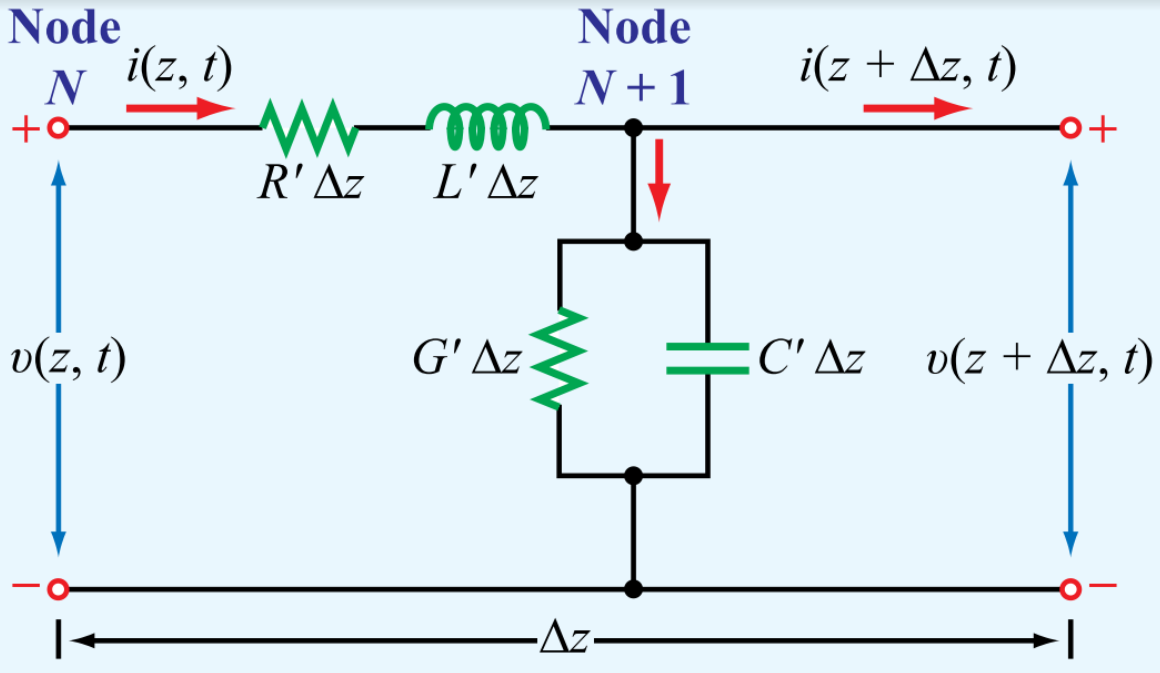
\includegraphics[scale=0.25]{lumped_elements.png}
		\end{center}
		\item lumped element model = transmission line is represented with L-network of $R', L', G',$ and $C'$ of length $\Delta z$. these are in per unit length elements (eg. $\Omega / m$)\\
		KVL analysis of the big loop: 
		\begin{align*}
			v(z,~t) = R'\Delta zi(z,~t) + L'\Delta z\diffp{i(z,~t)}{t} + v(z + \Delta z,~t) &\Longrightarrow -\diffp{v(z,~t)}{z} =  R'i(z,~t) + L'\diffp{i(z,~t)}{t} \\
		\end{align*}
		KCL at node $N+ 1$
		\begin{align*}
			i(z,~t) = G'\Delta v(z + \Delta z,~t) + C'\Delta z\diffp{v(z + \Delta z,~t)}{t} + i(z + \Delta z,~t) &\Longrightarrow -\diffp{i(z,~t)}{z} =  G'v(z,~t) + C'\diffp{v(z,~t)}{t} \\
		\end{align*}
		\item Telegrapher's equations: 
		\begin{align*}
			-\diffp{v(z,~t)}{z} &=  R'i(z,~t) + L'\diffp{i(z,~t)}{t} \\
			-\diffp{i(z,~t)}{z} &=  G'v(z,~t) + C'\diffp{v(z,~t)}{t}
		\end{align*}
		we define the following (as sinusoidal steady state transmission):
		\begin{align*}
			v(z,~t) &= \mathfrak{Re}\left\{V(z)\exp\left(j\omega t\right)\right\} \\
			i(z,~t) &= \mathfrak{Re}\left\{I(z)\exp\left(j\omega t\right)\right\}
		\end{align*}
		the telegrapher's equations become: 
		\begin{align*}
			-\diffp{v(z)}{z} &= \left(R' + j\omega L'\right)i(z) \numberthis \\
			-\diffp{i(z)}{z} &= \left(G' + j\omega C'\right)v(z) \numberthis
		\end{align*}
		differentiating (3) w. r. t. $z$ then combine with (4), and differentiate (4) w. r. t $z$ then combine with (3):
		\begin{align*}
			\diffp[2]{v(z)}{z} - \left(R' + j\omega L'\right)\left(G' + j\omega C'\right)v(z) &= 0 \\
			\diffp[2]{i(z)}{z} - \left(R' + j\omega L'\right)\left(G' + j\omega C'\right)i(z) &= 0
		\end{align*}
		let $\gamma = \sqrt{\left(R' + j\omega L'\right)\left(G' + j\omega C'\right)} = \alpha + j\beta$ \\
		the solutions are
		\begin{align*}
			v(z) &= V_0^f\exp\left(-\gamma z\right) + V_0^r\exp\left(\gamma z\right) \\
			i(z) &= I_0^f\exp\left(-\gamma z\right) + I_0^r\exp\left(\gamma z\right)	
		\end{align*}
		\item the relationship of $i(z)$ and $v(z)$: $i(z) = \frac{\gamma}{R' + j\omega L'}\left[V_0^f\exp\left(-\gamma z\right) - V_0^r\exp\left(-\gamma z\right)\right]$
		\item the characteristic impedance is $Z_0 = \frac{V_0^f}{I_0^f} = -\frac{V_0^r}{I_0^r} = \frac{R' + j\omega L'}{\gamma} = \sqrt{\frac{R' + j\omega L'}{G' + j\omega C'}}$
		\item the time domain expressions are:
		\begin{align*}
			v(z,~t) &= V_0^f\exp\left(-\alpha z\right)\cos\left(\omega t -\beta z\right) + V_0^r\exp\left(\alpha z\right)\cos\left(\omega t +\beta z\right) \\
			i(z,~t) &= I_0^f\exp\left(-\alpha z\right)\cos\left(\omega t -\beta z\right) + I_0^r\exp\left(\alpha z\right)\cos\left(\omega t +\beta z\right)
		\end{align*}
		\item the wavelength $\lambda = \frac{2\pi}{\beta}$
		\item the wavespeed $v_p = \frac{\omega}{\beta} = \lambda f$
		\item Lossless transmission lines: $R' = 0,~G' = 0$
			\begin{itemize}
				\item $\gamma = \sqrt{\left((0) + j\omega L'\right)\left((0) + j\omega C'\right)} = (0) + j\beta = j\omega\sqrt{L'C'}$
				\item $Z_0 = \sqrt{\frac{(0) + j\omega L'}{(0) + j\omega C'}} = \sqrt{\frac{L'}{C'}}$
				\item $v(z) = V_0^f\exp\left(-j\beta z\right) + V_0^r\exp\left(j\beta z\right)$
				\item $i(z) = I_0^f\exp\left(-j\beta z\right) + I_0^r\exp\left(j\beta z\right)$
				\item $\lambda = \frac{2\pi}{\omega\sqrt{L'C'}}$
				\item $v_p = \frac{1}{\sqrt{L'C'}}$
			\end{itemize}
		\item in a lossy transmission line with permeability $\mu$, surface resistance $R_S = \frac{1}{\sigma\delta_S}$, complex permittivity $\varepsilon = \varepsilon' - j\varepsilon''$:
			\begin{align*}
				W_m = \frac{\mu}{4}\int_S \bvec{H}_S \cdot \bvec{H}_S^* \dd S \Longrightarrow &L' = \frac{\mu}{\left|I_0\right|^2}\int_S \bvec{H}_S \cdot \bvec{H}_S^* \dd S \\
				W_e = \frac{\varepsilon}{4}\int_S \bvec{E}_S \cdot \bvec{E}_S^* \dd S \Longrightarrow &C' = \frac{\varepsilon'}{\left|V_0\right|^2}\int_S \bvec{E}_S \cdot \bvec{E}_S^* \dd S  \\
				&R' = \frac{R_S}{\left|I_0\right|^2}\int_{C1 + C2} \bvec{H}_S \cdot \bvec{H}_S^* \dd L \\
				&G' = \frac{\omega\varepsilon''}{\left|V_0\right|^2}\int_{S} \bvec{E}_S \cdot \bvec{E}_S^* \dd S \\
			\end{align*}
		\item terminanted transmission line. consider the case at which a lossless line is terminated by an impedance $Z_L$ at the receiving port and extends infinitely from one end. let the point where the load side connects with the transmission line be $z = 0$.
		\begin{align*}
			V(0) &= V_0 = V_0^f + V_0^r \\
			I(0) &= \frac{V_0}{Z_L} = \frac{V_0^f}{Z_0} - \frac{V_0^r}{Z_0} \\
			&\Big\Updownarrow \\
			V_0^f &= \frac{V_0}{2}\left(\frac{1}{Z_0} + \frac{1}{Z_l}\right) \\ 
			V_0^r &= \frac{V_0}{2}\left(\frac{1}{Z_0} - \frac{1}{Z_l}\right) \\ 
		\end{align*} 
		The current and voltage is: 
		\begin{align*}
			V(z) &= \frac{V_0}{2}\left(\frac{1}{Z_0} + \frac{1}{Z_l}\right)\exp\left(-j k z\right) + \frac{V_0}{2}\left(\frac{1}{Z_0} - \frac{1}{Z_l}\right)\exp\left(j k z\right) \\
			I(z) &= \frac{V_0}{2Z_0}\left(\frac{1}{Z_0} + \frac{1}{Z_l}\right)\exp\left(-j k z\right) + \frac{V_0}{2Z_0}\left(\frac{1}{Z_0} - \frac{1}{Z_l}\right)\exp\left(j k z\right)
		\end{align*}
		the relationship of the forward and reverse wave is $\frac{V_0^r}{V_0^f} = \frac{Z_L - Z_0}{Z_L + Z_0}$
		\item special cases:
		\begin{center}
			\begin{tabular}{|l|c|l|}
				\hline
				& Reflected Voltage & Remarks \\ \hline
				Open circuit ($Z_L \to \infty$) & $\frac{V_0^r}{V_0^f} = 1$ & same phase \\ \hline 
				Short circuit ($Z_L \to 0$) & $\frac{V_0^r}{V_0^f} = -1$ & $\pi$ out of phase \\ \hline 
				Matched load ($Z_L = Z_0$) & $\frac{V_0^r}{V_0^f} = 0$ & no reflection, maximum power transfer\\ \hline 
			\end{tabular}
		\end{center}
		\item Impedance transformation. using Ohm's law: $Z(z) = \frac{V(z)}{I(z)} = Z_0\frac{Z_L + jZ_0\tan\left(\beta z\right)}{Z_0 + jZ_L\tan\left(\beta z\right)}$
		\item at the quarter wavelength line (quarter wave transform), $z = \frac{\lambda}{4}, \beta = \frac{2\pi}{\lambda} \Longrightarrow\beta z = \frac{\pi}{2}$
		\begin{align*}
			Z_{eq} &= Z_0\frac{Z_L + jZ_0\tan\left(\frac{\pi}{2}\right)}{Z_0 + jZ_L\tan\left(\frac{\pi}{2}\right)} \\
			&\Big\Updownarrow \\
			Z_{eq}Z_L &= Z_0^2
		\end{align*}
		special cases: 
		\begin{center}
			\begin{tabular}{|l|c|l|}
				\hline
				& $Z_L$ &$ Z_{eq}$ \\ \hline
				Open circuit  & $\infty$ & 0 \\ \hline 
				Short circuit & $0$ & $\infty$ \\ \hline 
				Matched load  & $Z_0$ & $Z_0$\\ \hline 
			\end{tabular}
		\end{center}
	\end{enumerate}
\end{document}	
